\documentclass[11pt,a4paper]{article}
\usepackage{amsmath, amssymb, graphicx, xcolor}

\setlength{\textwidth}{6.8in}
\setlength{\textheight}{9.6in}
\setlength{\oddsidemargin}{-0.15in}
\setlength{\evensidemargin}{-0.15in}
\setlength{\topmargin}{-0.6in}
\setlength{\headheight}{0in}
\setlength{\headsep}{0in}
\setlength{\parindent}{0pt}
\setlength{\parskip}{5pt}

\definecolor{primary}{RGB}{15, 45, 95}
\definecolor{secondary}{RGB}{30, 80, 150}
\definecolor{accent}{RGB}{180, 40, 40}
\definecolor{qboxbg}{RGB}{245, 248, 252}
\definecolor{solboxbg}{RGB}{250, 250, 250}
\definecolor{rulecolor}{RGB}{210, 220, 235}

\newcommand{\questionheader}[3]{
    \vspace{0.35cm}
    \noindent\colorbox{qboxbg}{
        \parbox{\dimexpr\textwidth-2\fboxsep\relax}{
            \textbf{\textcolor{primary}{\large #1}} \hfill \textbf{\textcolor{accent}{[#2]}} \hfill \textbf{\textcolor{secondary}{#3 Marks}}
        }
    }
    \vspace{0.15cm}
}

\newcommand{\sectionbanner}[1]{
    \vspace{0.5cm}
    \noindent\colorbox{primary}{
        \parbox{\dimexpr\textwidth-2\fboxsep\relax}{
            \centering \textbf{\textcolor{white}{\Large #1}}
        }
    }
    \vspace{0.25cm}
}

\begin{document}

\begin{center}
    {\LARGE \textbf{\textcolor{primary}{BRAC UNIVERSITY}}}\\[4pt]
    {\large \textbf{Department of Computer Science and Engineering}}\\[3pt]
    {\textbf{CSE421 / EEE465: Computer Networks --- Final Examination}}\\[2pt]
    \textbf{Semester:} Fall 2025 \quad | \quad \textbf{Set:} A (v1) \quad | \quad \textbf{Full Marks:} 70 \quad | \quad \textbf{Duration:} 2 Hours\\[2pt]
    \rule{\textwidth}{1.5pt}
    {\large \textbf{\textcolor{secondary}{COMPREHENSIVE SOLUTION AND ANSWER KEY}}}
    \rule{\textwidth}{0.8pt}
\end{center}

\sectionbanner{SECTION A: MANDATORY QUESTIONS (40 MARKS)}

% =========================================================================
% QUESTION 1
% =========================================================================
\questionheader{Question 1: Subnetting \& Variable Length Subnet Masking (VLSM)}{CO3}{4 + 2 + 10 = 16}

\textbf{Problem Statement:}
A network consists of two subnets, referred to as \textbf{Network A} and \textbf{Network B}. Network A and Network B are consecutive subnets within the same major address block (i.e., there are no other subnets between them). Network A supports \textbf{1022 hosts}. A PC in Network A is assigned the first usable IP address of its subnet. This PC sends an IP packet with:
\begin{itemize}
    \item \textbf{Source IP address:} 172.16.8.1
    \item \textbf{Destination IP address:} 172.16.13.255
\end{itemize}
The packet is received by all devices in Network B.

\textbf{I. Determine the network (subnet) address of Network B. [4 Marks]}

\textbf{Solution:}
\begin{enumerate}
    \item \textbf{Analyze Network A:}
    \begin{itemize}
        \item Network A supports 1022 hosts.
        \item The number of host bits $h_A$ required satisfies:
        \[
        2^{h_A} - 2 \ge 1022 \implies 2^{h_A} \ge 1024 \implies h_A = 10\text{ bits}
        \]
        \item The prefix length for Network A is:
        \[
        32 - h_A = 32 - 10 = /22 \quad (\text{Subnet Mask: } 255.255.252.0)
        \]
        \item In a $/22$ subnet, the block size in the 3rd octet is $2^{10}/256 = 4$.
        \item The PC is assigned the first usable IP address: \texttt{172.16.8.1}.
        \item Since the first usable IP is formed by adding 1 to the network address, the \textbf{Network Address of Network A is \texttt{172.16.8.0/22}}.
        \item Therefore, Network A spans:
        \begin{itemize}
            \item Network Address: \texttt{172.16.8.0}
            \item Usable Host Range: \texttt{172.16.8.1} -- \texttt{172.16.11.254}
            \item Directed Broadcast Address: \texttt{172.16.11.255}
        \end{itemize}
    \end{itemize}

    \item \textbf{Analyze Network B:}
    \begin{itemize}
        \item The problem states Network A and Network B are \textbf{consecutive subnets} within the same address block with no subnets between them.
        \item Since Network A ends at \texttt{172.16.11.255}, Network B must begin immediately at the very next IP address:
        \[
        \text{\textbf{Network Address of Network B}} = \mathbf{172.16.12.0}
        \]
        \item The destination IP address of the packet is \texttt{172.16.13.255}. Since this packet is received by \emph{all devices in Network B}, \texttt{172.16.13.255} must be the \textbf{directed broadcast address} of Network B!
        \item The address range for Network B is from \texttt{172.16.12.0} to \texttt{172.16.13.255}, which spans $2 \times 256 = 512 = 2^9$ total IP addresses.
        \item Thus, Network B has $h_B = 9$ host bits and prefix length $32 - 9 = /23$ (Subnet Mask: \texttt{255.255.254.0}).
    \end{itemize}
\end{enumerate}
\textbf{Answer:} Subnet (Network) address of Network B is \textbf{\texttt{172.16.12.0/23}} (or \textbf{\texttt{172.16.12.0}}).

\vspace{0.2cm}
\textbf{II. Determine the maximum number of hosts that Network B can support. [2 Marks]}

\textbf{Solution:}
Network B has prefix length $/23$, which gives $h_B = 32 - 23 = 9$ host bits.
\[
\text{Maximum Usable Hosts} = 2^{h_B} - 2 = 2^9 - 2 = 512 - 2 = \mathbf{510\text{ hosts}}
\]
\textbf{Answer:} \textbf{510 hosts}.

\vspace{0.2cm}
\textbf{III. VLSM Subnetting for Given Topology. [10 Marks]}

\textbf{Problem Statement:}
Given the IP block \texttt{10.192.128.0/18}. Apply VLSM to identify the sub-network addresses for each subnet present in the figure shown. Note: The number of hosts given in the topology only includes the end devices.

\begin{center}
    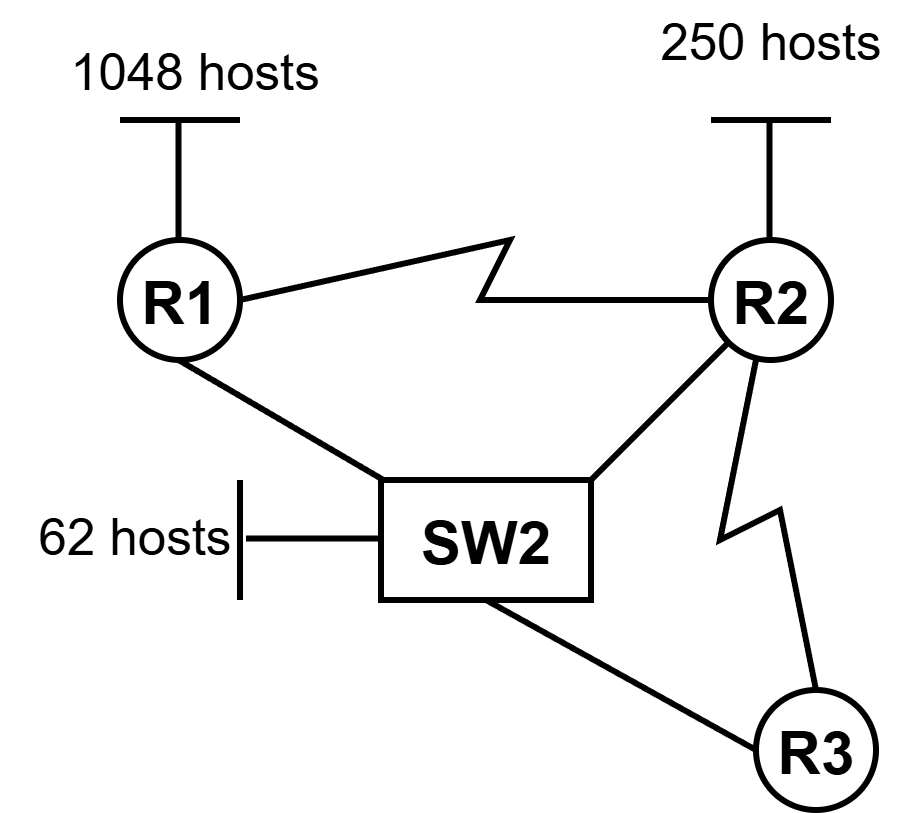
\includegraphics[width=0.36\textwidth]{p1_q1_topology.png}
\end{center}

\textbf{Step-by-Step Solution:}
\begin{enumerate}
    \item \textbf{Analyze Total Address Capacity of Major Block:}
    Major block: \texttt{10.192.128.0/18}. Total addresses $= 2^{32-18} = 2^{14} = 16,384$.
    
    \item \textbf{Count All Required IP Addresses (End Devices + Router Interfaces):}
    \begin{itemize}
        \item \textbf{Subnet 1 (R1 LAN):} 1048 end devices + 1 default gateway (R1 interface) = \textbf{1049 IP addresses}.
        \item \textbf{Subnet 2 (R2 LAN):} 250 end devices + 1 default gateway (R2 interface) = \textbf{251 IP addresses}.
        \item \textbf{Subnet 3 (SW2 Multi-Access LAN):} 62 end devices + 3 router interfaces (R1, R2, and R3 connect to SW2) = \textbf{65 IP addresses}.
        \item \textbf{Subnet 4 (WAN Link R1--R2):} Serial point-to-point link between R1 and R2 = \textbf{2 IP addresses}.
        \item \textbf{Subnet 5 (WAN Link R2--R3):} Serial point-to-point link between R2 and R3 = \textbf{2 IP addresses}.
    \end{itemize}

    \item \textbf{Order Requirements in Descending Order and Allocate Subnets:}
    \begin{itemize}
        \item \textbf{1st Allocation --- R1 LAN (Needs 1049 addresses):}
        \begin{itemize}
            \item $2^h - 2 \ge 1049 \implies 2^{10}-2 = 1022 < 1049 \implies h = 11$ bits ($2^{11} = 2048$ addresses).
            \item Prefix: $32 - 11 = /21$ (Subnet Mask: \texttt{255.255.248.0}). Block size in 3rd octet = 8.
            \item \textbf{Network Address:} \texttt{10.192.128.0/21}
            \item Usable Range: \texttt{10.192.128.1} to \texttt{10.192.135.254}
            \item Broadcast: \texttt{10.192.135.255}
            \item Next Available Base: \texttt{10.192.136.0}
        \end{itemize}

        \item \textbf{2nd Allocation --- R2 LAN (Needs 251 addresses):}
        \begin{itemize}
            \item $2^h - 2 \ge 251 \implies h = 8$ bits ($2^8 - 2 = 254 \ge 251$).
            \item Prefix: $32 - 8 = /24$ (Subnet Mask: \texttt{255.255.255.0}). Block size in 3rd octet = 1.
            \item \textbf{Network Address:} \texttt{10.192.136.0/24}
            \item Usable Range: \texttt{10.192.136.1} to \texttt{10.192.136.254}
            \item Broadcast: \texttt{10.192.136.255}
            \item Next Available Base: \texttt{10.192.137.0}
        \end{itemize}

        \item \textbf{3rd Allocation --- SW2 LAN (Needs 65 addresses):}
        \begin{itemize}
            \item $2^h - 2 \ge 65 \implies 2^6 - 2 = 62 < 65 \implies h = 7$ bits ($2^7 = 128$ addresses).
            \item Prefix: $32 - 7 = /25$ (Subnet Mask: \texttt{255.255.255.128}). Block size in 4th octet = 128.
            \item \textbf{Network Address:} \texttt{10.192.137.0/25}
            \item Usable Range: \texttt{10.192.137.1} to \texttt{10.192.137.126}
            \item Broadcast: \texttt{10.192.137.127}
            \item Next Available Base: \texttt{10.192.137.128}
        \end{itemize}

        \item \textbf{4th Allocation --- WAN Link R1--R2 (Needs 2 addresses):}
        \begin{itemize}
            \item $2^h - 2 \ge 2 \implies h = 2$ bits ($2^2 = 4$ addresses).
            \item Prefix: $32 - 2 = /30$ (Subnet Mask: \texttt{255.255.255.252}). Block size in 4th octet = 4.
            \item \textbf{Network Address:} \texttt{10.192.137.128/30}
            \item Usable Range: \texttt{10.192.137.129} to \texttt{10.192.137.130}
            \item Broadcast: \texttt{10.192.137.131}
            \item Next Available Base: \texttt{10.192.137.132}
        \end{itemize}

        \item \textbf{5th Allocation --- WAN Link R2--R3 (Needs 2 addresses):}
        \begin{itemize}
            \item $h = 2$ bits $\implies$ Prefix: $/30$ (Subnet Mask: \texttt{255.255.255.252}).
            \item \textbf{Network Address:} \texttt{10.192.137.132/30}
            \item Usable Range: \texttt{10.192.137.133} to \texttt{10.192.137.134}
            \item Broadcast: \texttt{10.192.137.135}
        \end{itemize}
    \end{itemize}
\end{enumerate}

\textbf{Summary Table of Allocated Subnets:}
\begin{center}
\begin{tabular}{|l|c|c|c|l|l|}
\hline
\textbf{Subnet Name} & \textbf{Req. Hosts} & \textbf{Allocated} & \textbf{Prefix} & \textbf{Network Address} & \textbf{Usable Range} \\
\hline
R1 LAN & 1048+1=1049 & 2046 & /21 & \texttt{10.192.128.0} & \texttt{10.192.128.1} -- \texttt{10.192.135.254} \\
R2 LAN & 250+1=251 & 254 & /24 & \texttt{10.192.136.0} & \texttt{10.192.136.1} -- \texttt{10.192.136.254} \\
SW2 LAN & 62+3=65 & 126 & /25 & \texttt{10.192.137.0} & \texttt{10.192.137.1} -- \texttt{10.192.137.126} \\
WAN R1--R2 & 2 & 2 & /30 & \texttt{10.192.137.128} & \texttt{10.192.137.129} -- \texttt{10.192.137.130} \\
WAN R2--R3 & 2 & 2 & /30 & \texttt{10.192.137.132} & \texttt{10.192.137.133} -- \texttt{10.192.137.134} \\
\hline
\end{tabular}
\end{center}

\newpage
% =========================================================================
% QUESTION 2
% =========================================================================
\questionheader{Question 2: IPv4 Fragmentation \& Path MTU Discovery}{CO2, CO3}{3 + 3 + 4 + 3 = 13}

\textbf{Problem Statement:}
A network-layer PDU of \textbf{4680 bytes}, including a \textbf{20-byte header}, is fragmented for transmission over a link with an MTU of \textbf{X bytes}. The difference between the fragment offset values of two consecutive fragments is \textbf{75}. The fragment offset of the first fragment is 0.

\textbf{I. Calculate the value of MTU (X). [3 Marks]}

\textbf{Solution:}
\begin{itemize}
    \item Total original datagram size $= 4680$ bytes.
    \item IPv4 header size $= 20$ bytes. Total payload/data size $= 4680 - 20 = 4660$ bytes.
    \item The Fragment Offset field in an IPv4 header measures data offset in \textbf{8-byte units} (scale factor of 8).
    \item Given difference between consecutive fragment offsets: $\Delta \text{Offset} = 75$.
    \item Therefore, the payload/data size carried by each non-terminal fragment is:
    \[
    \text{Data per fragment} = 75 \times 8 = \mathbf{600\text{ bytes}}
    \]
    \item Each fragment transmitted over the link includes the 20-byte IP header. Hence, the total fragment size is:
    \[
    \text{Fragment Size} = 600 + 20 = 620\text{ bytes}
    \]
    \item In IP fragmentation, the maximum data payload must be the largest multiple of 8 such that $\text{Data} + 20 \le \text{MTU}$. Therefore, the link MTU $X$ is \textbf{$620 \le X < 628$ bytes}, with the standard nominal value being:
    \[
    \mathbf{X = 620\text{ bytes}}
    \]
\end{itemize}

\textbf{II. Calculate the fragment offset of the 4th fragment. [3 Marks]}

\textbf{Solution:}
\begin{itemize}
    \item From the course networking formulas, the Fragment Offset for the $k$-th fragment is given directly by:
    \[
    \text{Fragment Offset}_k = \frac{(k - 1) \times \text{Payload}}{8}
    \]
    where $k$ is the fragment index ($k = 1, 2, 3, \dots$) and $\text{Payload}$ is the data payload size per full fragment.
    \item Here, $k = 4$ and $\text{Payload} = 600\text{ bytes}$ (with $\frac{\text{Payload}}{8} = \Delta\text{Offset} = 75$):
    \[
    \text{Offset}_4 = \frac{(4 - 1) \times 600}{8} = \frac{3 \times 600}{8} = 3 \times 75 = \mathbf{225}
    \]
    \item (Verification: The 4th fragment carries data starting at byte offset $225 \times 8 = 1800$, spanning bytes 1800 to 2399).
\end{itemize}
\textbf{Answer:} Fragment offset of the 4th fragment is \textbf{225}.

\vspace{0.2cm}
\textbf{III. Calculate the data size of the last fragment. [4 Marks]}

\textbf{Solution:}
\begin{itemize}
    \item Total original payload data $= 4660$ bytes.
    \item Data payload in each full fragment $= 600$ bytes.
    \item Number of full fragments $= \lfloor 4660 / 600 \rfloor = 7$ fragments.
    \item Total data in the first 7 fragments $= 7 \times 600 = 4200$ bytes.
    \item The remaining data carried in the 8th (last) fragment is:
    \[
    \text{Data size of last fragment} = 4660 - 4200 = \mathbf{460\text{ bytes}}
    \]
    \item (Verification: Total size of last fragment $= 460 + 20 = 480\text{ bytes} \le 620$; Fragment offset $= 4200/8 = 525$; More Fragments flag $MF = 0$).
\end{itemize}
\textbf{Answer:} \textbf{460 bytes}.

\vspace{0.2cm}
\textbf{IV. If the DF value of the original datagram was set, how was the packet sent to its destination? [3 Marks]}

\textbf{Solution:}
\begin{itemize}
    \item If the \textbf{DF (Don't Fragment)} bit is set to 1 ($DF = 1$), the intermediate router is strictly prohibited from fragmenting the datagram.
    \item Since the original datagram size (4680 bytes) exceeds the link MTU (620 bytes), the router \textbf{drops/discards the packet}.
    \item The router sends an \textbf{ICMP Destination Unreachable message} (\textbf{Type 3, Code 4:} \emph{"Fragmentation Needed and DF set"}) back to the source host. This ICMP message includes the Next-Hop MTU (620 bytes).
    \item Upon receiving this message, the source host performs \textbf{Path MTU Discovery (PMTUD)}. It reduces its segment size (TCP MSS) so that packets do not exceed 620 bytes, and retransmits the data as smaller individual datagrams that require no fragmentation along the path.
\end{itemize}

\newpage
% =========================================================================
% QUESTION 3
% =========================================================================
\questionheader{Question 3: DHCPv4, Link-Layer Operations, \& ARP Inter-Subnet Flow}{CO2}{2 + 3 + 3 + 3 = 11}

\begin{center}
    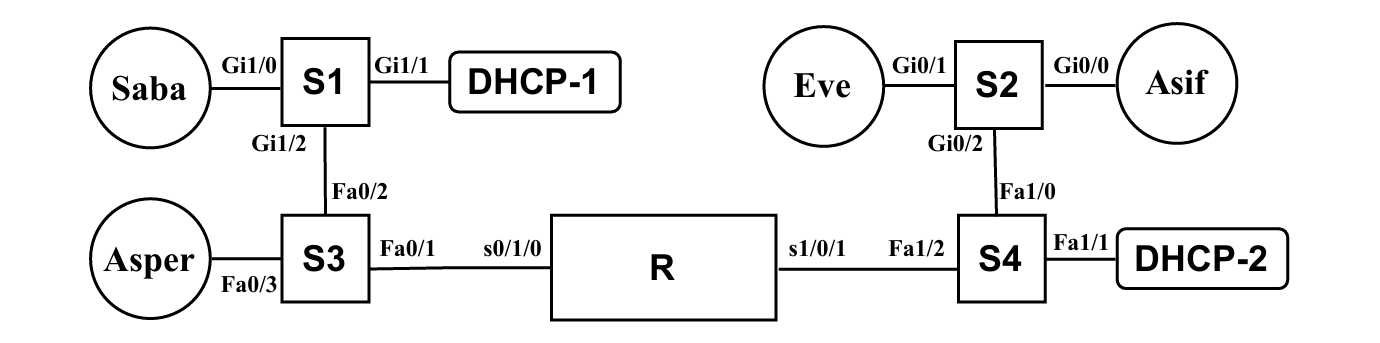
\includegraphics[width=0.85\textwidth]{p1_q3_topology.png}
\end{center}

\textbf{Context:} Saba and Eve have just connected to their networks. All switches have empty MAC tables; MAC aging time is 2 minutes. MAC address of each host is its name (e.g., ASIF).

\textbf{I. Saba’s PC sends its first DHCP message to obtain an IP address. What source IP address is used in this packet? [2 Marks]}

\textbf{Solution:}
\begin{itemize}
    \item Saba's initial DHCP message is a \textbf{DHCPDISCOVER} message.
    \item At this point, Saba does not have an IP address configured.
    \item Therefore, the IPv4 source address used in the IP header is \textbf{\texttt{0.0.0.0}} (representing \emph{"this host on this network"}).
    \item (The destination IP is the limited broadcast address \texttt{255.255.255.255}, with UDP source port 68 and destination port 67).
\end{itemize}
\textbf{Answer:} \textbf{\texttt{0.0.0.0}}.

\vspace{0.2cm}
\textbf{II. Asper connects at the same time as Saba and sends a DHCP request. How can DHCP-1 distinguish Saba’s request from Asper’s request even though both requests are broadcast? [3 Marks]}

\textbf{Solution:}
DHCP-1 distinguishes between the two broadcast requests using the following fields:
\begin{enumerate}
    \item \textbf{Client Hardware Address (\texttt{chaddr}) in DHCP Payload:} The DHCP application-layer message contains the client's Layer 2 hardware address. Saba's request specifies \texttt{chaddr = SABA}, whereas Asper's request specifies \texttt{chaddr = ASPER}.
    \item \textbf{Transaction ID (\texttt{xid}):} Each client independently generates a random 32-bit transaction identifier (\texttt{xid}) that uniquely correlates the discovery, offer, request, and acknowledgment messages.
    \item \textbf{Layer 2 Ethernet Header Source MAC:} Even though the destination MAC is broadcast (\texttt{FF:FF:FF:FF:FF:FF}), the source MAC in the Ethernet frame header is the sender's individual physical address (\texttt{SABA} vs. \texttt{ASPER}).
\end{enumerate}

\vspace{0.2cm}
\textbf{III. Eve has used an address from DHCP-2 for 5 hours. Her renewal attempt to DHCP-2 fails, but she then successfully obtains a new address from DHCP-1. Briefly explain how Eve is able to obtain an IP address from DHCP-1. [3 Marks]}

\textbf{Solution:}
\begin{enumerate}
    \item When the unicast renewal attempt to DHCP-2 fails (at timer $T_1 = 50\%$), Eve reaches the rebinding timer ($T_2 = 87.5\%$ of lease time) and enters the \textbf{REBINDING} state. In this state, Eve broadcasts a DHCPREQUEST to find \emph{any} active DHCP server on the network.
    \item However, DHCP-1 is on a completely different subnet separated by Router R. Under normal circumstances, routers block broadcast frames (\texttt{255.255.255.255}).
    \item To allow Eve to reach DHCP-1, Router R must be configured as a \textbf{DHCP Relay Agent} (e.g., using \texttt{ip helper-address <IP\_of\_DHCP-1>} on interface \texttt{s1/0/1} / \texttt{Fa1/2}).
    \item Router R intercepts Eve's broadcast message, converts it into a unicast UDP packet (setting \texttt{giaddr} to Router R's interface IP on Eve's subnet), and forwards it across the router to DHCP-1.
    \item DHCP-1 recognizes that the request originates from Eve's subnet via \texttt{giaddr}, assigns an appropriate IP from its configured address pool for that subnet, and returns the response via Router R.
\end{enumerate}

\vspace{0.2cm}
\textbf{IV. Asper intends to send a packet to Eve. Since Eve is on a different subnet, Asper must send the packet to Router R. Name the specific link-layer requests and responses that are exchanged between Asper and Router R to make this possible? [3 Marks]}

\textbf{Solution:}
\begin{enumerate}
    \item \textbf{ARP Request (Broadcast):} Asper determines by subnet masking that Eve's IP is on a remote subnet. Therefore, Asper must forward the frame to its Default Gateway (Router R's interface connected to switch S3). Since Asper does not have Router R's MAC address in its ARP cache, Asper broadcasts an \textbf{ARP Request}:
    \begin{itemize}
        \item Frame Source MAC: \texttt{ASPER}, Destination MAC: \texttt{FF:FF:FF:FF:FF:FF}
        \item ARP Payload: \emph{"Who has IP address of Router R? Tell Asper."}
    \end{itemize}
    \item \textbf{ARP Reply (Unicast):} Router R receives the broadcast ARP request, records Asper's IP-to-MAC mapping, and returns a unicast \textbf{ARP Reply}:
    \begin{itemize}
        \item Frame Source MAC: \texttt{MAC\_R} (Router R's S3 interface), Destination MAC: \texttt{ASPER}
        \item ARP Payload: \emph{"Router R's IP is at MAC\_R."}
    \end{itemize}
    \item Once Asper receives the ARP Reply, Asper caches Router R's MAC address and encapsulates the IP datagram addressed to Eve into an Ethernet frame with Destination MAC = \texttt{MAC\_R}.
\end{enumerate}

\newpage
\sectionbanner{SECTION B: ANY TWO OUT OF THREE (12 MARKS)}
\textit{(All questions solved below for comprehensive coverage)}

% =========================================================================
% QUESTION 4
% =========================================================================
\questionheader{Question 4: Static Routing Configuration \& Floating Static Routes}{CO3}{3 + 3 = 6}

\begin{center}
    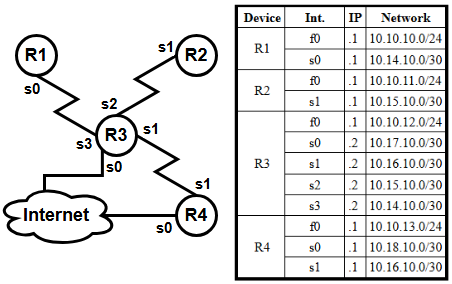
\includegraphics[width=0.55\textwidth]{p1_q4_topology.png}
\end{center}

\textbf{Context:} Each router has a LAN connected to its \texttt{f0} interface.
\begin{itemize}
    \item R1: \texttt{f0} (10.10.10.1/24), \texttt{s0} (10.14.10.1/30) $\to$ connects to R3 \texttt{s3} (10.14.10.2/30)
    \item R2: \texttt{f0} (10.10.11.1/24), \texttt{s1} (10.15.10.1/30) $\to$ connects to R3 \texttt{s2} (10.15.10.2/30)
    \item R3: \texttt{f0} (10.10.12.1/24), \texttt{s0} (10.17.10.2/30), \texttt{s1} (10.16.10.2/30), \texttt{s2} (10.15.10.2/30), \texttt{s3} (10.14.10.2/30)
    \item R4: \texttt{f0} (10.10.13.1/24), \texttt{s0} (10.18.10.1/30), \texttt{s1} (10.16.10.1/30) $\to$ connects to R3 \texttt{s1} (10.16.10.2/30)
\end{itemize}

\textbf{I. Configure a non-recursive static route to R2 LAN from R4. [3 Marks]}

\textbf{Solution:}
\begin{itemize}
    \item Destination Network: R2 LAN = \texttt{10.10.11.0/24} (Subnet Mask: \texttt{255.255.255.0}).
    \item A \textbf{non-recursive static route} (directly attached static route) specifies the \textbf{exit interface} directly instead of a next-hop IP address (eliminating recursive route lookups in the routing table).
    \item On router R4, the outbound interface towards R3 (and thus to R2) is serial interface \textbf{\texttt{s1}}.
    \item Cisco IOS configuration command on R4:
    \begin{center}
        \texttt{R4(config)\# ip route 10.10.11.0 255.255.255.0 s1}
    \end{center}
    \textit{(Note: A fully specified static route specifying both exit interface and next hop: \texttt{ip route 10.10.11.0 255.255.255.0 s1 10.16.10.2} also avoids recursive lookup).}
\end{itemize}

\vspace{0.2cm}
\textbf{II. Assume R4 is routing to all unknown routes to the internet via s0. Configure a floating static route for this route. [3 Marks]}

\textbf{Solution:}
\begin{itemize}
    \item The primary default route to the Internet on R4 is configured via interface \texttt{s0}:
    \begin{center}
        \texttt{R4(config)\# ip route 0.0.0.0 0.0.0.0 s0} \quad (\text{Administrative Distance } AD = 1)
    \end{center}
    \item A \textbf{floating static route} serves as an automatic backup route that appears in the routing table only when the primary link fails. It is created by assigning an \textbf{Administrative Distance (AD) strictly greater than 1} (e.g., AD = 10 or 200).
    \item If R4's direct internet link \texttt{s0} fails, R4 can reach the Internet via \textbf{R3} (which also has a direct connection to the Internet on its \texttt{s0} interface). The next-hop IP on R3 is \texttt{10.16.10.2} via interface \texttt{s1}.
    \item Cisco IOS configuration command on R4:
    \begin{center}
        \texttt{R4(config)\# ip route 0.0.0.0 0.0.0.0 10.16.10.2 10}
    \end{center}
    \textit{(or with interface and next-hop: \texttt{R4(config)\# ip route 0.0.0.0 0.0.0.0 s1 10.16.10.2 10})}.
\end{itemize}

% =========================================================================
% QUESTION 5
% =========================================================================
\questionheader{Question 5: IPv6 Address Representation \& Multicast Principles}{CO3}{3 + 3 = 6}

\textbf{I. Expand the following IPv6 Addresses in their Hexadecimal form: [3 Marks]}

\textbf{Solution:}
An uncompressed IPv6 address consists of 8 groups (hextets) of 4 hexadecimal digits (total 128 bits):
\begin{enumerate}
    \item \textbf{A. \texttt{FE80::1A2B}}
    \begin{itemize}
        \item Present groups: \texttt{FE80} and \texttt{1A2B} (2 groups).
        \item The double colon \texttt{::} represents $8 - 2 = 6$ consecutive groups of zeros.
        \item Padding leading zeros to 4 hex digits per group:
        \[
        \mathbf{fe80:0000:0000:0000:0000:0000:0000:1a2b}
        \]
    \end{itemize}

    \item \textbf{B. \texttt{2001:DB8:1234::10}}
    \begin{itemize}
        \item Present groups: \texttt{2001}, \texttt{0db8}, \texttt{1234} and \texttt{0010} (4 groups).
        \item The double colon \texttt{::} replaces $8 - 4 = 4$ groups of zeros.
        \[
        \mathbf{2001:0db8:1234:0000:0000:0000:0000:0010}
        \]
    \end{itemize}

    \item \textbf{C. \texttt{::25}}
    \begin{itemize}
        \item Present group: \texttt{0025} (1 group at the end).
        \item The double colon \texttt{::} replaces $8 - 1 = 7$ groups of zeros.
        \[
        \mathbf{0000:0000:0000:0000:0000:0000:0000:0025}
        \]
    \end{itemize}
\end{enumerate}

\vspace{0.2cm}
\textbf{II. A PC sends a packet to 224.10.10.5, but only some PCs receive it. Explain why. [3 Marks]}

\textbf{Solution:}
\begin{itemize}
    \item The address \texttt{224.10.10.5} belongs to \textbf{IPv4 Class D} (\texttt{224.0.0.0} to \texttt{239.255.255.255}), designated specifically for \textbf{Multicast Addressing}.
    \item Multicast operates on a \textbf{one-to-many subscription model}: a packet sent to a multicast group address is not delivered to everyone on the network (which would be a broadcast), but only to hosts that have explicitly joined that multicast group.
    \item Hosts join a multicast group by signaling their local router using the \textbf{Internet Group Management Protocol (IGMP)}.
    \item Modern switches run \textbf{IGMP Snooping}, which maps multicast MAC/IP groups to specific switch ports. Traffic destined for \texttt{224.10.10.5} is forwarded only to switch ports connected to subscribed hosts.
    \item PCs that have not joined \texttt{224.10.10.5} ignore or filter out the frames at their Network Interface Card (NIC), which is why only member PCs receive the packet.
\end{itemize}

% =========================================================================
% QUESTION 6
% =========================================================================
\questionheader{Question 6: Switch Self-Learning \& Frame Processing}{CO2}{3 + 3 = 6}

\textbf{Context:} Refer to the network diagram in Question 3.
\begin{itemize}
    \item Saba $\to$ S1 (\texttt{Gi1/0}); DHCP-1 $\to$ S1 (\texttt{Gi1/1}); S1--S3 link: S1 (\texttt{Gi1/2}) to S3 (\texttt{Fa0/2})
    \item Asper $\to$ S3 (\texttt{Fa0/3}); S3 $\to$ Router R: S3 (\texttt{Fa0/1}) to R (\texttt{s0/1/0})
    \item Router R $\to$ S4: R (\texttt{s1/0/1}) to S4 (\texttt{Fa1/2}); DHCP-2 $\to$ S4 (\texttt{Fa1/1}); S4--S2 link: S4 (\texttt{Fa1/0}) to S2 (\texttt{Gi0/2})
    \item Eve $\to$ S2 (\texttt{Gi0/1}); Asif $\to$ S2 (\texttt{Gi0/0})
\end{itemize}

\textbf{I. Asif wants to send an IP packet to Eve, but does not yet know Eve’s MAC address. What frame does Asif generate (source and destination MAC), and how do the switches S1, S2, S3, and S4 process this frame? [3 Marks]}

\textbf{Solution:}
\begin{enumerate}
    \item \textbf{Frame Generated by Asif:}
    Since Asif needs Eve's MAC address, Asif generates an \textbf{ARP Request}:
    \begin{itemize}
        \item \textbf{Source MAC:} \texttt{ASIF}
        \item \textbf{Destination MAC:} \texttt{FF:FF:FF:FF:FF:FF} (Broadcast MAC)
    \end{itemize}

    \item \textbf{Processing by Switch S2:}
    \begin{itemize}
        \item The broadcast frame enters S2 on port \texttt{Gi0/0}.
        \item \textbf{Self-Learning:} S2 records in its MAC table: \texttt{MAC: ASIF} $\to$ \texttt{Port: Gi0/0}.
        \item \textbf{Forwarding:} Since destination MAC is broadcast, S2 floods the frame out of all other active interfaces: \texttt{Gi0/1} (towards Eve) and \texttt{Gi0/2} (towards S4).
        \item Eve receives the ARP Request on \texttt{Gi0/1}.
    \end{itemize}

    \item \textbf{Processing by Switch S4:}
    \begin{itemize}
        \item S4 receives the broadcast frame on port \texttt{Fa1/0} from S2.
        \item \textbf{Self-Learning:} S4 records in its MAC table: \texttt{MAC: ASIF} $\to$ \texttt{Port: Fa1/0}.
        \item \textbf{Forwarding:} S4 floods the frame out of all other ports: \texttt{Fa1/1} (to DHCP-2) and \texttt{Fa1/2} (to Router R).
    \end{itemize}

    \item \textbf{Processing by Router R, S3, and S1:}
    \begin{itemize}
        \item Router R receives the broadcast frame on its interface \texttt{s1/0/1}. Routers terminate Layer 2 broadcast domains and \textbf{do NOT forward broadcast frames}.
        \item Therefore, the frame is dropped by Router R and \textbf{never reaches S3 or S1}.
        \item \textbf{Switches S3 and S1 do not process the frame at all}, and their MAC tables remain completely empty.
    \end{itemize}
\end{enumerate}

\vspace{0.2cm}
\textbf{II. After Eve replies to Asif, show the MAC address tables of all the switches. [3 Marks]}

\textbf{Solution:}
\begin{enumerate}
    \item \textbf{Eve's ARP Reply:}
    Eve generates a unicast ARP reply with:
    \begin{itemize}
        \item \textbf{Source MAC:} \texttt{EVE}
        \item \textbf{Destination MAC:} \texttt{ASIF}
    \end{itemize}
    \item \textbf{Processing by Switch S2:}
    \begin{itemize}
        \item The frame enters S2 on port \texttt{Gi0/1}.
        \item S2 learns: \texttt{MAC: EVE} $\to$ \texttt{Port: Gi0/1}.
        \item S2 looks up destination MAC \texttt{ASIF} in its MAC table and finds a known entry (\texttt{Gi0/0}).
        \item S2 forwards the frame \textbf{directly and solely out of port \texttt{Gi0/0}} to Asif.
        \item S2 does \textbf{NOT} flood the frame; therefore, the reply is \textbf{never forwarded to S4}.
    \end{itemize}
\end{enumerate}

\textbf{Final MAC Tables of All Switches:}

\begin{center}
\begin{tabular}{|c|c|}
\multicolumn{2}{c}{\textbf{Switch S1}} \\
\hline
\textbf{MAC Address} & \textbf{Port} \\
\hline
\multicolumn{2}{|c|}{\textit{(Empty --- No frames reached S1)}} \\
\hline
\end{tabular}
\quad
\begin{tabular}{|c|c|}
\multicolumn{2}{c}{\textbf{Switch S2}} \\
\hline
\textbf{MAC Address} & \textbf{Port} \\
\hline
\texttt{ASIF} & \texttt{Gi0/0} \\
\texttt{EVE}  & \texttt{Gi0/1} \\
\hline
\end{tabular}
\quad
\begin{tabular}{|c|c|}
\multicolumn{2}{c}{\textbf{Switch S3}} \\
\hline
\textbf{MAC Address} & \textbf{Port} \\
\hline
\multicolumn{2}{|c|}{\textit{(Empty --- No frames reached S3)}} \\
\hline
\end{tabular}
\quad
\begin{tabular}{|c|c|}
\multicolumn{2}{c}{\textbf{Switch S4}} \\
\hline
\textbf{MAC Address} & \textbf{Port} \\
\hline
\texttt{ASIF} & \texttt{Fa1/0} \\
\hline
\end{tabular}
\end{center}

\newpage
\sectionbanner{SECTION C: ANY THREE OUT OF FIVE (18 MARKS)}
\textit{(All questions solved below for comprehensive coverage)}

% =========================================================================
% QUESTION 7
% =========================================================================
\questionheader{Question 7: IPv4 Time-to-Live (TTL) \& ICMP Smurf Attack}{CO2}{3 + 3 = 6}

\textbf{I. Apart from limiting the number of hops, explain how the Time to Live (TTL) field helps prevent network problems. What would happen to the Internet if the TTL field did not exist? [3 Marks]}

\textbf{Solution:}
\begin{itemize}
    \item \textbf{Role of TTL:}
    In an IP network, temporary routing loops can arise due to slow routing protocol convergence, misconfigurations, or link state changes. If a packet enters a routing loop, it circulates endlessly between routers. The 8-bit TTL field is decremented by 1 by each router that processes the datagram. When TTL reaches 0, the packet is discarded, and an ICMP \emph{Time Exceeded} message (Type 11, Code 0) is returned to the source.
    \item \textbf{Consequences if TTL Did Not Exist:}
    \begin{enumerate}
        \item \textbf{Endless Circulation of Packets:} Without TTL, looping packets would circulate permanently across the network infrastructure.
        \item \textbf{Exponential Congestion Collapse:} As new packets continuously enter existing loops, link bandwidth and router memory buffers would become completely saturated.
        \item \textbf{Total Internet Breakdown:} Legitimate packets would be dropped due to buffer overflow, leading to catastrophic network-wide starvation and the collapse of Internet routing.
    \end{enumerate}
\end{itemize}

\vspace{0.2cm}
\textbf{II. An attacker discovers a network with 200 active devices. He sends one ICMP Echo Request in such a way that the target victim receives 200 ICMP Echo Replies. How is it possible? [3 Marks]}

\textbf{Solution:}
This attack is an ICMP-based amplification Denial-of-Service attack known as a \textbf{Smurf Attack}:
\begin{enumerate}
    \item \textbf{IP Source Address Spoofing:} The attacker crafts a single ICMP Echo Request (ping packet) and sets the \textbf{Source IP} to the \textbf{Victim's IP address}.
    \item \textbf{Directed Broadcast Destination:} The attacker sends this packet with the \textbf{Destination IP} set to the \textbf{directed broadcast address} of the target subnet (e.g., \texttt{192.168.1.255} for a $/24$ subnet containing 200 active devices).
    \item \textbf{Amplification by Local Hosts:} The edge router broadcasts the packet over the local link. All 200 active devices receive the ICMP Echo Request and each responds with an ICMP Echo Reply destined to the spoofed source IP (the victim).
    \item Thus, from a single packet transmitted by the attacker, the victim is bombarded by \textbf{200 simultaneous ICMP Echo Replies}.
\end{enumerate}

% =========================================================================
% QUESTION 8
% =========================================================================
\questionheader{Question 8: Heterogeneous Routing Protocols \& Count-to-Infinity}{CO3}{3 + 3 = 6}

\textbf{Problem Statement:}
Suppose Router R1 and R3 in Q4's topology are using the Distance Vector Routing Algorithm, while routers R2 and R4 are using the Link State routing Protocol. Suddenly, the link between R1 and R3 fails.

\textbf{I. Explain whether this link failure will cause the count-to-infinity problem. [3 Marks]}

\textbf{Solution:}
\begin{itemize}
    \item \textbf{No, this link failure will NOT cause the count-to-infinity problem.}
    \item \textbf{Technical Justification:}
    \begin{enumerate}
        \item The \textbf{Count-to-Infinity problem} occurs in Distance Vector routing when two or more routers form a cyclic path/loop (e.g., mutually advertising an unreachable network to one another with progressively increasing hop counts).
        \item In Q4's topology, R1 connects solely to R3 via link \texttt{s0}--\texttt{s3} (a single point-to-point stub link). R1 has no other neighboring routers running Distance Vector.
        \item When the link between R1 and R3 fails, R1 has \textbf{no alternate path} and no other neighbor to exchange Distance Vector routing tables with.
        \item Furthermore, R2 and R4 are running Link State (OSPF) rather than Distance Vector; without route redistribution, Distance Vector advertisements cannot circulate through R2 or R4.
        \item Therefore, R3 immediately detects the link loss, sets the metric to R1's network to $\infty$ (16 in RIP), and purges it. No cyclic counting can occur.
    \end{enumerate}
\end{itemize}

\vspace{0.2cm}
\textbf{II. Once the link between R1 and R3 fails, all routers have only their directly connected networks in their routing tables. Explain the reason. [3 Marks]}

\textbf{Solution:}
\begin{itemize}
    \item \textbf{Protocol Incompatibility without Route Redistribution:}
    R1 and R3 run a Distance Vector protocol (e.g., RIP), while R2 and R4 run a Link State protocol (e.g., OSPF). Routing protocols do not natively share routes across different protocol domains. Unless \textbf{mutual route redistribution} is explicitly configured on the boundary router (R3), routes from one protocol domain are invisible to the other.
    \item \textbf{Impact of Link Failure on the Topology:}
    \begin{enumerate}
        \item \textbf{Router R1:} Completely isolated. Its only dynamic routing adjacency was with R3. With the link severed, it flushes all learned routes and retains only its directly connected LAN (\texttt{f0}).
        \item \textbf{Router R3:} Acts as the central hub. When the link to R1 fails, it loses its only Distance Vector peer. If R3 is not configured to redistribute routes into OSPF, or if the failure disrupts routing processes, dynamic routes are not propagated.
        \item \textbf{Routers R2 and R4:} Connected only via R3 in the core. If R3 does not run Link State on all its interfaces or fails to form proper adjacencies with R2 and R4, R2 and R4 cannot learn each other's LANs.
        \item Consequently, dynamic route entries time out and are purged, leaving all routers with \textbf{only their directly connected interfaces}.
    \end{enumerate}
\end{itemize}

\newpage
% =========================================================================
% QUESTION 9
% =========================================================================
\questionheader{Question 9: Port Address Translation (PAT) \& Inbound Traversal}{CO2}{3 + 3 = 6}

\textbf{Context:}
Hosts A and D inside a LAN communicate with remote host B through an edge router performing PAT. The edge router has \texttt{220.20.20.17/30} in its PAT pool.
\begin{itemize}
    \item Packet from Host A to Host B: Source IP \texttt{192.168.2.105}, Source Port \texttt{52157}, Dest IP \texttt{6.6.6.6}, Dest Port \texttt{344}.
    \item Packet from Host D to Host B: Source IP \texttt{192.168.2.106}, Source Port \texttt{52157}, Dest IP \texttt{6.6.6.6}, Dest Port \texttt{344}.
\end{itemize}

\textbf{I. Identify the source IP and port address of the packets sent by host A and host D when they leave the edge router for host B. [3 Marks]}

\textbf{Solution:}
\begin{itemize}
    \item \textbf{PAT Pool Analysis:} The address block is \texttt{220.20.20.17/30}. For a $/30$ subnet, the network address is \texttt{220.20.20.16}, and usable public IP addresses are \textbf{\texttt{220.20.20.17}} and \textbf{\texttt{220.20.20.18}}.
    \item \textbf{Packet from Host A:}
    \begin{itemize}
        \item The router translates Host A's private IP to the first public IP \texttt{220.20.20.17}.
        \item Since port 52157 is free on this public IP, PAT preserves the source port:
        \item \textbf{Source IP:} \texttt{220.20.20.17}, \textbf{Source Port:} \texttt{52157}.
    \end{itemize}
    \item \textbf{Packet from Host D:}
    \begin{itemize}
        \item Host D is communicating with the exact same destination (\texttt{6.6.6.6:344}) using the same private source port \texttt{52157}.
        \item The socket tuple \texttt{(220.20.20.17, 52157, 6.6.6.6, 344)} is already allocated to Host A.
        \item \textbf{PAT must resolve this collision} using either of two standard mechanisms:
        \begin{enumerate}
            \item \textbf{Port Multiplexing on Same IP:} Allocate the next available ephemeral port:
            \[
            \textbf{Source IP: } \texttt{220.20.20.17}, \quad \textbf{Source Port: } \mathbf{52158} \text{ (or other unique port } \ne 52157)
            \]
            \item \textbf{Using the Second Pool IP:}
            \[
            \textbf{Source IP: } \texttt{220.20.20.18}, \quad \textbf{Source Port: } \mathbf{52157}
            \]
        \end{enumerate}
    \end{itemize}
\end{itemize}

\vspace{0.2cm}
\textbf{II. Suppose a remote host C on the Internet wants to initiate new communication with host A. Explain why or why not this would be possible with the current setup. If not, how can it be made possible? [3 Marks]}

\textbf{Solution:}
\begin{itemize}
    \item \textbf{Why it is NOT possible under the current setup:}
    \begin{itemize}
        \item PAT is inherently \textbf{stateful and outbound-driven}. Translation table entries are created dynamically only when an inside host initiates an outbound session.
        \item When remote host C initiates an unsolicited inbound packet, the edge router looks up its NAT/PAT state table.
        \item Because no corresponding translation entry exists, the router does not know which internal private host to forward the packet to, and \textbf{discards the packet}.
    \end{itemize}
    \item \textbf{How it can be made possible:}
    \begin{enumerate}
        \item \textbf{Port Forwarding (Static PAT):} Configure a static mapping on the router mapping an external port (e.g., \texttt{220.20.20.17:8080}) to Host A's internal IP and port (\texttt{192.168.2.105:8080}).
        \item \textbf{1:1 Static NAT:} Dedicate the second public IP address in the pool (\texttt{220.20.20.18}) exclusively to Host A (\texttt{192.168.2.105}).
        \item \textbf{DMZ (Demilitarized Zone):} Configure Host A as the default DMZ host to receive all unsolicited incoming traffic.
    \end{enumerate}
\end{itemize}

% =========================================================================
% QUESTION 10
% =========================================================================
\questionheader{Question 10: IPv6 Transition, Anycast Addressing, \& Extension Headers}{CO2, CO3}{1 + 2 + 3 = 6}

\textbf{Scenario 1:} An organization needs IPv6 devices to communicate with IPv4 devices during the transition period.\\
\textbf{Scenario 2:} A service is deployed using the same IPv6 address on multiple routers. Clients always reach the nearest router automatically.

\textbf{I. Name the IPv6 transition technique used in Scenario 1. [1 Mark]}

\textbf{Solution:}
\textbf{NAT64 / DNS64} (or \textbf{Dual-Stack} / \textbf{NAT-PT: Network Address Translation -- Protocol Translation}).

\vspace{0.2cm}
\textbf{II. What IPv6 addressing mechanism is used in Scenario 2? Is there any difference between this mechanism and multicast addressing? [2 Marks]}

\textbf{Solution:}
\begin{itemize}
    \item \textbf{Addressing Mechanism:} \textbf{Anycast Addressing} (one-to-nearest).
    \item \textbf{Difference from Multicast Addressing:}
    \begin{itemize}
        \item \textbf{Anycast (One-to-One-of-Many):} The same address is assigned to multiple interfaces across different devices. A packet sent to an anycast address is routed to \textbf{only one single node} --- the topologically nearest node as determined by the routing protocol.
        \item \textbf{Multicast (One-to-Many):} A packet sent to a multicast address is delivered to \textbf{all nodes} that belong to the multicast group.
    \end{itemize}
\end{itemize}

\vspace{0.2cm}
\textbf{III. IPv6 does not have an Options field like IPv4. Since the IPv6 base header is fixed at 40 bytes, mention how IPv6 carries additional information when required. [3 Marks]}

\textbf{Solution:}
\begin{itemize}
    \item IPv6 replaces the variable-length IPv4 Options field with \textbf{Extension Headers}.
    \item Extension headers are inserted between the fixed 40-byte IPv6 base header and the upper-layer payload (e.g., TCP/UDP).
    \item They form a flexible \textbf{daisy chain} using the \textbf{Next Header} field:
    \begin{itemize}
        \item The base header's \texttt{Next Header} field specifies the type of the first extension header.
        \item Each extension header contains its own \texttt{Next Header} field pointing to the next extension header or the transport-layer protocol.
    \end{itemize}
    \item Key Extension Headers include:
    \begin{enumerate}
        \item \textbf{Hop-by-Hop Options Header:} Processed by every router on the path (e.g., jumbo payloads).
        \item \textbf{Routing Header:} Directs the packet through specified intermediate routers (source routing).
        \item \textbf{Fragment Header:} Handles packet fragmentation at the sending source host.
        \item \textbf{Encapsulating Security Payload (ESP) \& Authentication Header (AH):} Provides IPSec encryption and integrity.
    \end{enumerate}
\end{itemize}

% =========================================================================
% QUESTION 11
% =========================================================================
\questionheader{Question 11: MAC Address Classification \& Structural Properties}{CO2}{3 + 3 = 6}

\textbf{I. Rahim wants to understand how to determine whether a given MAC address is unicast or multicast. Explain how he can identify this from the MAC address. [3 Marks]}

\textbf{Solution:}
\begin{itemize}
    \item A standard IEEE 802 MAC address is 48 bits (6 bytes) long, represented as 12 hexadecimal digits: \texttt{XX:XX:XX:XX:XX:XX}.
    \item Unicast vs. Multicast is defined by the \textbf{Least Significant Bit (LSB) of the First Octet} (known as the \textbf{I/G bit --- Individual/Group}):
    \[
    \text{First Byte: } b_7 b_6 b_5 b_4 b_3 b_2 b_1 \mathbf{b_0}
    \]
    \begin{itemize}
        \item If $b_0 = \mathbf{0}$: The address is \textbf{Individual (Unicast)}.
        \item If $b_0 = \mathbf{1}$: The address is \textbf{Group (Multicast / Broadcast)}.
    \end{itemize}
    \item \textbf{Hexadecimal Rule of Thumb:} Look at the \textbf{second hexadecimal digit} of the MAC address:
    \begin{itemize}
        \item If the 2nd hex digit is \textbf{EVEN} (\texttt{0, 2, 4, 6, 8, A, C, E}), the MAC address is \textbf{Unicast} (e.g., \texttt{0\textbf{0}:1A:2B:3C:4D:5E}).
        \item If the 2nd hex digit is \textbf{ODD} (\texttt{1, 3, 5, 7, 9, B, D, F}), the MAC address is \textbf{Multicast} (e.g., \texttt{0\textbf{1}:00:5E:00:00:01}).
    \end{itemize}
\end{itemize}

\vspace{0.2cm}
\textbf{II. His friend remarked that MAC addresses are hierarchical and portable. Justify whether his friend's remark about MAC addresses is correct. [3 Marks]}

\textbf{Solution:}
His friend's remark is \textbf{partially correct and partially incorrect}:
\begin{enumerate}
    \item \textbf{Portable --- CORRECT:}
    MAC addresses are physical (burned-in) hardware addresses burned into the Network Interface Card (NIC). A device retains the exact same MAC address regardless of what physical network, subnet, or geographic location it is moved to. Therefore, MAC addresses are truly \textbf{portable}.
    \item \textbf{Hierarchical --- INCORRECT (in a Networking Context):}
    \begin{itemize}
        \item IP addresses are hierarchical (Network ID + Subnet ID + Host ID), allowing routers to summarize millions of destinations into compact routing entries based on topological location.
        \item In contrast, MAC addresses are \textbf{flat} with respect to network topology.
        \item Although a MAC address has an administrative structure (the first 24 bits are the IEEE OUI identifying the vendor, and the remaining 24 bits are the serial number), this structure conveys \textbf{no geographical or topological routing information}. A switch cannot aggregate MAC addresses by network location.
        \item Hence, in the context of network routing and addressing architecture, MAC addresses are \textbf{flat, not hierarchical}.
    \end{itemize}
\end{enumerate}

\begin{center}
    \rule{\textwidth}{0.8pt}\\[3pt]
    \textbf{\textcolor{primary}{--- END OF EXAMINATION SOLUTION ---}}
\end{center}

\end{document}
